\section{Grundlagen}

\begin{frame}{Grundlagen - Beugung von Wellen}
    \centering
    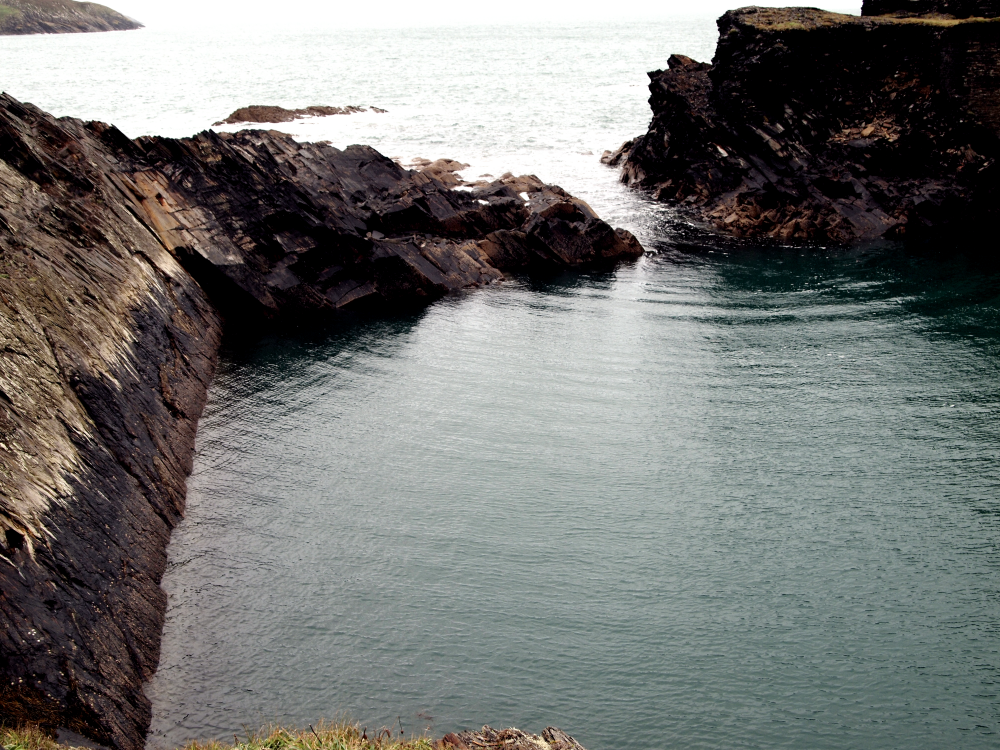
\includegraphics[height=0.9\textheight]{images/beugung_von_wasserwellen.png}
\end{frame}

\begin{frame}{Grundlagen - Prinzip von Huygens}
    \includegraphics[width=\linewidth]{../../SeminarHarmonischeAnalysis/buch/papers/opt/images/huygens.pdf}
\end{frame}

\begin{frame}{Grundlagen - Beugung beim JWST}
    \begin{columns}
        \begin{column}{0.4\textwidth}
            \centering
            \includegraphics[width=\textwidth, page = 1]{../../SeminarHarmonischeAnalysis/buch/papers/opt/images/jwst_sechseck.pdf}
            Beugung am Spiegel
        \end{column}
        \pause
        \begin{column}{0.4\textwidth}
            \centering
            \includegraphics[width=\textwidth, page = 2]{../../SeminarHarmonischeAnalysis/buch/papers/opt/images/jwst_sechseck.pdf}
            Beugung an den Streben
        \end{column}
    \end{columns}
\end{frame}

\begin{frame}[plain]
    \begin{tikzpicture}[overlay, remember picture]
        \node[inner sep=0pt] at (current page.center)
        {\includegraphics[height=\pdfpagewidth]{../../SeminarHarmonischeAnalysis/buch/papers/opt/images/jamesWebb_publicDomain.png}};
    \end{tikzpicture}
\end{frame}

\begin{frame}{Grundlagen - Problemstellung}
    \begin{columns}
        \begin{column}{0.3\textwidth}
            \includegraphics[width=\linewidth, trim={8cm, 1cm, 0, 0}, clip]{../../SeminarHarmonischeAnalysis/buch/papers/opt/images/huygens.pdf}
        \end{column}
        \begin{column}{0.7\textwidth}
            \includegraphics[width=\linewidth]{../../SeminarHarmonischeAnalysis/buch/papers/opt/images/derivation.pdf}
        \end{column}
    \end{columns}

    \begin{block}<2->{Ziel}
        Berechnen der Überlagerung aller Wellen am Auswertungspunkt $P(x_p, y_p)$.

        \begin{itemize}
            \item<3-> Wie kann eine Welle beschrieben werden?
            \item<4-> Wie verhält sich das elektrische Feld?
        \end{itemize}
    \end{block}
\end{frame}

\begin{frame}{Grundlagen - Wellendarstellung}
    \begin{columns}
        \begin{column}{0.5\textwidth}
            \begin{center}
                \includegraphics[width=\linewidth]{../../SeminarHarmonischeAnalysis/buch/papers/opt/images/welle.pdf}
            \end{center}
        \end{column}
        \begin{column}{0.5\textwidth}
            \begin{block}<1->{Differentialgleichung}
                \begin{equation*}
                    \frac{\partial^2\zeta(x, t)}{\partial t^2}
                    =
                    u^2 \cdot \frac{\partial^2\zeta(x, t)}{\partial x^2}
                \end{equation*}
            \end{block}
            \begin{block}<2->{\strut Welle aus Physik 3 \cite{opt:HSR:Physik2}}
                \begin{align*}
                    \zeta(x, t)
                    &=
                    \zeta_0 \cdot \sin(\omega t - \vec{k}\cdot\vec{x})
                    \\
                    k
                    &=
                    \frac{\omega}{u}
                    =
                    \frac{2 \pi}{\lambda}
                \end{align*}
            \end{block}
            \begin{exampleblock}<3->{Komplexwertiger Zeiger}
                \begin{equation*}
                    \zeta(x, t)
                    =
                    \zeta_0 \cdot e^{j(\omega t - \vec{k}\cdot\vec{x})}      
                \end{equation*}
            \end{exampleblock}
        \end{column}
    \end{columns}
\end{frame}

\begin{frame}{Grundlagen - Elektrische Feldstärke}
    \begin{columns}
        \begin{column}{0.5\textwidth}
            \begin{center}
                \includegraphics[width=\linewidth]{../../SeminarHarmonischeAnalysis/buch/papers/opt/images/maxwell.pdf}
            \end{center}
        \end{column}

        \begin{column}{0.5\textwidth}
            \begin{block}{Erste Maxwellsche Gleichung}
                \begin{align*}
                    \oint_{S=\partial V} \varepsilon\vec{E} \cdot\, d\vec{S}
                    &=
                    \int_{V}\rho\, dV
                    \\
                \end{align*}
            \end{block}
            \pause
            \begin{block}{Angewandt}
                \begin{align*}
                    \int_{0}^{a}\int_{0}^{2\pi} \varepsilon E\cdot 1 \cdot r\, d\varphi dl
                    &=
                    Q
                    \\
                    2\pi ra\varepsilon E
                    &=
                    Q
                \end{align*}
            \end{block}
            \pause
            \begin{exampleblock}{Elektrische Feldstärke}
                \begin{equation*}
                    E(r)
                    =
                    \frac{Q}{2\pi\varepsilon a} \cdot \frac{1}{r}
                    =
                    C \cdot \frac{1}{r}
                \end{equation*}
            \end{exampleblock}
        \end{column}
    \end{columns}
\end{frame}
